\documentclass[a4paper,12pt]{article}

\usepackage[french]{babel}
\usepackage[utf8]{inputenc}
\usepackage{graphicx}
\usepackage{textcomp}
\usepackage{lscape}
\usepackage{amsmath}
\usepackage{moreverb}
\usepackage{hyperref}
\hypersetup{colorlinks, citecolor=black, filecolor=black, linkcolor=black, urlcolor=black}
\usepackage{fancyhdr}

\title{Projet Nigma : Première soutenance}
\author{CrypTeam : LAPÔTRE Guillaume (\texttt{lapotr\_g}) \and GANIVET Justin (\texttt{ganive\_j}) \and LADEVIE Stéphane (\texttt{ladevi\_s}) \and GISLAIS Sébastien (\texttt{gislai\_s})}
\date{11 février 2009}

\pagestyle{myheadings}

\begin{document}

\markright{Première soutenance du Projet Nigma par la Crypteam}

\maketitle

\newpage

\tableofcontents

\newpage

\section{Introduction}

Voici une petite fiction pour observer le Projet Nigma en situation réelle :

Rappelons nous ce célèbre passage du Secret de l'Espadon, la première et la plus belle aventure de Black \& Mortimer (bande dessinée écrit et scénarisé par Edgar P. Jacobs) où le Capitaine Hasso agent de l'Intelligence Service qui, après une réunion de l'état major de l'empereur Basam-Damdu, se précipite dans sa chambre afin de communiquer d'importantes informations aux services secrets Britanniques à l'aide d'un radio émetteur minable. Il lui faut bien 10 minutes pour le régler et il a à peine le temps de révéler une partie de son message que le Colonel Olrik le surprend et l'abat d'une balle dans le dos.

On peut supposer qu'avec la totalité du message, les Anglais aurait pu se préparer bien mieux pour faire face à l'invasion \og jaune \fg{} Supposons que ce scénario se soit déroulé dans une autre époque, l'ère du numérique : le capitaine Hasso aurait certainement disposé d'un NetBook dernier cri sur lequel il aurait pu saisir toutes ses notes durant la réunion. Puis, il aurait rejoins sa chambre pour transmettre le fruit de son travail aux Anglais mais là il ne prend plus aucun risque grâce à la dernière acquisition des services secrets Britanniques : le Projet Nigma !

En effet grâce à ce programme révolutionnaire le courageux capitaine n'aurait qu'à lancer le programme pour crypter les données récoltées et les cacher dans une photo de vacance où on le voit avec ses 5 enfants et sa magnifique femme (personne n'a pensé à la famille du pauvre capitaine Hasso lorsqu'il s'est fait explosé le dos par le vil Olrik). Cette opération prend à peine une minute. Il n'aurait eu par la suite qu'à poster cette photo modifiée sur son FaceBook (tout le monde a un FaceBook, non ?) et les services secrets auraient récupéré toutes ces précieuses informations en consultant simplement le profil FaceBook du capitaine. Le colonel Olrik aurait alors surpris le capitaine Hasso en train de consulter son profil et, à moins de réellement haïr les réseaux sociaux, il n'aurait pas tué l'espion à la solde les Anglais.

Le monde aurait été certainement détruit de la même manière mais le capitaine Hasso serait vivant, il n'aurait pas laissé une veuve et 5 orphelins et il aurait certainement reçu une magnifique médaille pour services rendus. Faute de sauver le monde, la Crypteam sauve au moins une vie\dots{}

\begin{center}
  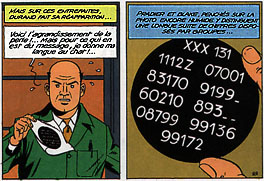
\includegraphics[scale=3]{meteores2.jpg}
\end{center}

Voici à présent le rapport de la première soutenance du Projet Nigma (Projet d'Info Spé EPITA promotion 2012) de la Crypteam. Nous vous rappelons que le Projet Nigma est un programme informatique de cryptage et de stéganographie dont l'objectif et la protection et la diffusion d'information sur des supports graphiques comme des photos ou des dessins, ce qui le rend utile sur une plateforme internationale comme l'Internet. Ce programme fusionne l'art du secret et l'art de la dissimulation pour offrir une sécurité maximum à l'utilisateur.

ATTENTION : Tout acquéreur d'un logiciel Projet Nigma endosse l'en\-tière responsabilité de ses activités mettant en usage ledit logiciel. La Crypteam ne saurait être tenu pour responsable en cas d'utilisation malhonnête, l'équipe ne fournit qu'un instrument.

\newpage

\section{Cryptographie}

Au niveau de la cryptographie, nous nous sommes tenu  ce que nous avions prévu dans le cahier des charges. Nous avons donc réalisé le cryptage RSA en Ocaml. Ce cryptage nous a posé plus de difficultées que prévu. Au tout début nous pensions que recoder le RSA était une chose difficile dans la mesure où c'est un algorithme de chiffrement encore utilisé aujourd'hui donc encore efficace (bien qu'inventé en 1977) puis en se documentant sur la façon dont fonctionne le RSA cela nous a paru relativement simple. En effet sa sécurité est basée sur la difficulté de factoriser un très grand nombre et non pas sur la difficulté à chiffrer/déchiffrer un document.

En effet le RSA est un procédé cryptographique asymétrique (ou bien à clé publique), ce qui veut dire qu'au lieu de générer une clé qui permet de chiffrer ainsi que de déchiffrer un message, le RSA génère une clé dite \og publique \fg{} ainsi qu'une clé dite \og privée \fg{}. Ces deux clés sont intimement liées. Cela veut dire que le RSA génère obligatoirement un couple comportant une clé publique ainsi qu'une clé privée en même temps. La fabrication de la clé privée dépend de la clé publique.

La clé publique est, comme son nom l'indique publique\dots{} C'est à dire que l'on peut la partager avec autant de personne que l'on désire. Cette clé permet de chiffrer un message. Par contre une fois le document chiffré, le document n'est déchiffrable que par le détenteur de la clé privée. Ainsi la personne qui a chiffré le message ne peut vérifier si le chiffrement c'est bien déroulé. Cette clé est un couple de deux nombres $(n, e)$ avec $n$ représentant le produit de deux grands nombres premiers, appelés $p$ et $q$, de l'ordre de plusieurs centaines de chiffres ! Et $e$ est un nombre premier avec le produit $(p - 1)(q - 1)$. Pour chiffrer un texte à l'aide de la clé il faut représenter notre message sous la forme d'un ou de plusieurs entiers $M_{i}$ compris entre $1$ et $n - 1$. Le message chiffré est représenté sous la forme des $C_{i} = M_{i}^e \mod n$.

La clé privée est la clé permettant de déchiffrer un message chiffré à l'aide de sa clé publique associée. Elle est donc gardée par son propriétaire. Elle est composée elle aussi d'un couple de nombre $(n, d)$. $n$ est identique au $n$ de la clé publique. Et $d$ est tel que $ed \equiv 1 \textrm{ mod } (p - 1)(q - 1)$. Pour déchiffrer un message la procédure est pratiquement identique au chiffrement : On calcule les $D_{i}$ tel que : $D_{i} = C_{i}^d \mod n$.

On remarque que le $e$ et le $d$ sont fabriqué à partir des nombres premiers $p$ et $q$. Si l'on pouvait facilement et rapidement factorisé notre $n$ afin de trouver $p$ et $q$ alors le RSA ne servirait plus à rien. C'est précisément parce qu'ils sont premiers et très grands qu'il est difficile de factoriser $n$.

\subsection{Partie de Guillaume Lapôtre}

J'ai tout d'abord commencé par essayer de créer mes grands nombres premiers puisqu'ils sont le fondement de la cryptographie RSA. J'ai rencontré quelques problèmes au début car je n'avais pas prévu que les entiers étaient représentés sur 31 bits en Ocaml. Ainsi lorsque je voulais créer un grand nombre, Ocaml plantait.

J'ai donc fait des recherches afin de trouver comment gérer des grands nombres en OCaml. J'ai trouvé deux modules satisfaisant à savoir Numerix et \texttt{Big\_int}. Numerix n'est pas une bibliothèque native de OCaml mais je l'ai trouvée intéressante car elle comportait déja une fonction pouvant determiner si un nombre est premier ou non. L'inconvenient non-négligeable est que ces tests de primalité sont efficaces pour un $n < 2^{50}$ or nous voulons des entiers premiers d'au moins un millier de bits. Du coup cette bibliothèque ne nous était plus utile et nous nous sommes rabattus sur la deuxième : \texttt{Big\_int}. Cette dernière à l'avantage d'être une bibliothèque native de Ocaml, ce qui nous permet de l'utiliser sans problème, sans installation supplémentaire au préalable.

\texttt{Big\_int} est donc une bibliothèque multi-précision gérant de grands entiers. On peut faire tout ce que l'on faisait déjà avec des entiers mais le nom des fonctions est différent. Le \emph{léger} inconvénient est que les opérateurs fonctionnent en préfixe. Cela implique que toutes les opérations que nous écrivons manipulant des \texttt{Big\_int} sont en notation polonaise.

Une fois compris comment s'appliquent la plupart des fonctions de la bibliothèque \texttt{Big\_int} je me suis intéressé une fois de plus à la création de mes grand nombres premiers. Pour tester si un $n$ est premier, l'algorithme le plus naïf est de tester si aucun $1 < p < \sqrt{n}$ ne divise $n$ nommé algorithme d'Euclide. Cet algorithme, comme celui  du crible d'Ératosthène, est beaucoup trop long pour trouver si un nombre de plusieurs centaines de chiffres est premier. Il existe donc plusieurs algorithmes plus évolués qui sont tous basés plus ou moins sur le petit théorème de Fermat : Si $p$ est un nombre premier et $a \in N $ alors $a^{p - 1} \equiv 1 \mod p$. Ce sont des algorithmes probabilistes, autrement dit lorsque l'on donne un nombre à ce type d'algorithme, il répond soit \og ce nombre est \emph{probablement} premier \fg{} soit \og ce nombre est composé \fg{}. Donc lorsque l'algorithme renvoie vrai on n'a pas la certitude que ce nombre est réellement premier. Heureusement ils répondent avec un certain degré de probabilité. Il existe 3 ou 4 algorithmes probabilistes pouvant être utilisé pour le RSA. Parmi eux il y a Solovay-Strassen, Lehmann, Miller-Rabin.

Cependant j'ai eut beaucoup de difficultées à coder ces algorithmes en OCaml. J'ai donc laissé cette partie à l'autre membre du groupe traitant la cryptographie : Sébastien Gislais. Il expliquera mieux que moi ses péripéties avec les nombres premiers.

Je suis donc passé à la suite du projet pour le RSA, donc à la création de mes nombres $e$ et $d$. La fonction générant $e$ n'a pas posé trop de souci du fait de sa définition relativement simple. Le nombre $d$ a été un peu plus fastidieux à générer du fait lui aussi de sa définition. Cependant après quelques recherches sur des sites Internet expliquant l'algorithme d'Euclide étendu ainsi que dans un livre de la bibliothèque d'EPITA nommé \textit{Cryptographie appliquée} je réussis à générer mon $d$. Ayant désormais tous les éléments constituant mes clés privée et publique, je voulais les écrire dans un fichier. Ainsi j'aurais mon fichier avec la clé privée que je conserve jalousement et mon fichier avec la clé publique que je partage avec toutes les personnes voulant m'envoyer un message chiffré. J'ai été agréablement surpris par la facilité de la gestion des fichiers par OCaml. J'ai ainsi créé mes clés sans problème.

Une fois mes clés générées, il me fallait maintenant faire le principal : chiffrer et déchiffrer un message. Nous voulions crypter avant tout du texte, mes clés étant numériques il fallait donc que je transforme mon texte en une suite de nombres. J'ai donc travaillé sur le code ASCII de mes caractères. Ainsi ma fonction de chiffrage a besoin de la clé publique ainsi que d'un fichier à crypter. Elle récupère chaque code ASCII de chaque caractère du fichier, chiffre ces caractères et met le résultat chiffré dans un nouveau fichier. Ce fichier chiffré est donc constitué d'une liste de codes ASCII chiffrés en RSA. Enfin, pour déchiffrer ce fichier, je déchiffre chaque caractère ASCII à l'aide de la clé privée et j'écris le caractère correspondant dans un nouveau fichier. Ainsi, je peux vérifier que le fichier d'origine et le fichier chiffré puis déchiffré sont identiques !
%Parler ensuite des stratégies pour gérer les fichiers : liste etc...

\newpage

\subsection{Partie de Sébastien Gislais}

J'ai démarré le projet en venant en aide à Guillaume. Il était très déconte\-nancé de ne pas pouvoir manipuler de grands entiers avec Caml. Nous avons testé la bibliothèque Numérix mais comme dit plus haut, les entiers gérés n'étaient pas si grands que ça. La bibliothèque par défaut de Caml nous a finalement paru bien utile : \texttt{Big\_int}. Ça présision arbitraire sur les entiers nous a en premier lieu permis de nous lancer dans la programmation de l'algorithme RSA.

La première étape de cet algorithme est de générer les nombres premiers $p$ et $q$ avec plusieurs centaines de chiffres pour rendre le chiffrage extrêmement difficile à casser. L'algorithme d'Euclide pour trouver des nombres premiers de cette taille est tout naturellement exclu. Nous avons trouvé, avec l'aide de notre professeur de mathématiques \textsc{M. Rodot}, les tests de primalités de Solovay-Strassen, de Lehmann et de Miller-Rabin dans le livre \textit{Cryptographie appliquée}. Nous allons présenter ces différents algorithmes probabilistes de test de primalité.

Le test de Solovay-Strassen utilise le symbole de \textsc{Jacobi} pour tester si $p$ est premier. Il est ainsi formulé :
\begin{enumerate}
\item Choississez un nombre aléatoire $a$ inférieur à $p$.
\item Si le $pgcd(a,p) \ne 1$, alors $p$ échoue au test et il est composé.
\item Calculer $j = a^{(p - 1) / 2} \mod p$.
\item Calculer le symbole de \textsc{Jacobi} $J(a,p)$.
\item Si $j \ne J(a,p)$, alors $p$ n'est certainement pas premier.
\item Si $j = J(a,p)$, alors la probabilité que $p$ ne soit pas premier est au plus de 50\,\%.
\end{enumerate}

Si on répète le test $k$ fois avec $k$ valeurs différentes aléatoires, un nombre composé a \emph{une} chance sur $2^k$ de passer les $k$ tests, soit une probabilité de $2^{-k}$ d'être certain que $p$ est un nombre premier. Avec 100 tests, nous sommes assez sûrs\dots{}

L'algorithme semble très alléchant, cependant, c'est lors de l'implantation du symbole de \textsc{Jacobi} que nous avons eu de petits problèmes.

Définition du symbole de \textsc{Jacobi} $J(a,n)$ pour $n$ impair :

\begin{displaymath}
J(a,n) =
\left\{
  \begin{array}{cc}
    1 & a = 1 \\
    J\left(\frac{a}{2}, n\right)(- 1)^{\frac{n^2 - 1}{8}} & a \textrm{ pair} \\
    J(n \mod a, a)(- 1)^{\frac{(a - 1) (n - 1)}{4}} & a \textrm{ impair}
  \end{array}
\right.
\end{displaymath}

L'implantation en Caml est on ne peut plus triviale par sa définition même, mais notre fonction récursive arrive à nous renvoyer des exceptions Caml \texttt{Out\_of\_memory} à la fin des retours d'appels, cela malgré l'utilisation des \texttt{Big\_int} et que le symbole de \textsc{Jacobi} ne renvoie que les valeurs $\{- 1, 0, 1\}$. Une exponentiation modulaire dans la puissance $(- 1)$ nous tira d'affaire après maintes recherches et tests. Heureusement que nous avons eu un séminaire Caml l'année dernière !

Nous ne sommes pas arrivés au bout de nos peines car l'implantation de l'algorithme de Solovay-Strassen nous a été impossible du fait de l'inférence de type. En effet, le typage fort de Caml ne nous a pas permis de renvoyer un résultat après nos boucles et nos tests de conditions de sortie.

\bigskip

Non découragés pour autant par ces deux retards, et forts de notre expé\-rience en algorithmique et en Caml, nous nous sommes littéralement attaqués à l'algorithme de Miller-Rabin que \og tout le monde utilise \fg{} d'après notre livre et Internet. Bref, tout le monde était au courant sauf nous\dots{} Il se présente sous cette forme :

Au préalable, il faut choisir un nombre aléatoire $p$ à tester et calculer $b$ tel que $b$ est le nombre de fois que 2 divise $p - 1$ (c'est-à-dire que $2^b$ est la plus grande puissance de 2 qui divise $p - 1$. Ensuite nous devons calculer $m$ tel que $p = 1 + 2^{b}m$.

\begin{enumerate}
\item Choisissez un nombre aléatoire $a$ inférieur à $p$.
\item Posez $j = 0$ et $z = a^{m} \mod p$.
\item Si $z = 1$ ou $z = p - 1$, alors $p$ passe le test et peut être premier.
\item Si $j > 0$ et $z = 1$, alors $p$ n'est pas premier.
\item Posez $j = j + 1$. Si $j < b$ et $z \ne p - 1$, posez $z = z^{2} \mod p$ et retournez à l'étape précédente. Si $z = p - 1$, alors $p$ passe le test et peut être premier.
\item Si $j = b$ et $z \ne p - 1$, alors $p$ n'est pas premier.
\end{enumerate}

Il fallut là encore imaginer, concevoir et innover pour implanter cet algorithme de Miller-Rabin. Le chemin fut hardu, encore à cause de l'inférence de type qui ne nous laisse pas tout faire. Nous avons dû utiliser et traduire en Caml des implantations de l'algorithme de Miller-Rabin depuis des scripts Python, du C, du C++ et autres langages de programmation. Les réflexes acquis par l'écriture du précédant algorithme de Solovay-Strassen ont aidé sans nul doute à ma réussite de l'homme sur la machine. J'eu raison de Caml qui est désormais soumis à notre volonté. Les nombres premiers à plusieurs \emph{centaines} de chiffres n'ont plus de secrets pour moi et peuvent être découverts très rapidement.

Les tests sont vraiment satisfaisants et concluants sur l'efficacité de mon implantation de l'algorithme : il faut moins de 4 minutes pour un processeur à double c\oe{}ur pour générer deux nombres premiers de 512 chiffres qui sont ensuite multipliés entre eux pour former un nombre de plus de 1024 chiffres ! Je rappelle qu'un nombre de 1024 chiffres est représenté en binaire par 3400 bits.

De nos jours, il est conseillé d'utiliser des clés de plus de 1024 bits pour le chiffrement RSA. En 2005, le plus grand nombre factorisé, selon l'état de l'art en matière de calculs distribués, était long de 663 bits. Seul un \emph{ordinateur quantique} peut factoriser un de nos nombres généré dans un temps humainement raisonnable ! Nous nous satifaisons de cette véritable performance.

\newpage

\section{Stéganographie}
\subsection{Partie Explication Stéganographie}

La stéganographie est l'art de cacher un message secret. Dans le projet Nigma, nous cachons ce message dans une image. Les images que nous utilisons pour le moment sont au format BMP. Le format BMP est constitué d'un header qui sert d'en-tête au fichier. Ce header fait 54 octets. Il est très important car il permet de connaitre les propriétés du fichier et de l'image comme le nombre de bits par pixel ou la taille de l'image. Il ne faut surtout pas toucher à ce header sinon l'image de base sera modifiée voire même illisible pour les logiciels de visualisation. Ainsi quand nous lisons l'image, nous sautons ces 54 octets qu'il ne faut pas toucher et nous les écrivons tels quels dans la future image.

Pour l'instant, ne nous pouvons cacher que du texte et pas un fichier en entier. Ce texte est une chaine de caractères que nous découpons caractère par caractère. Prenons l'exemple de l'astérisque : '*' sa valeur en ASCII est 42. En binaire cela fait donc \%101010. Un caractère fait 8 bits donc il faut rajouter un 0 à gauche. Cela nous donne \%0101010. Enfin nous rajoutons un 0 pour qu’un caractère soit codé sur 9 bits. Ainsi chaque caractère sera contenu dans 3 pixels puisque nous pouvons cacher 1 caractère dans un pixel.

Cette transformation faite, nous mettons cette chaine de bits sous la forme de chaîne de caractères. Ainsi '*' sera représenté sous la string "00101010". Nous répétons l'opération pour chaque caractère de la chaine et nous concaté\-nons le tout.

Que faire avec cette chaine de caractères exclusivement constitués de '0' et de '1' Et bien nous allons tout d'abord prendre caractère par caractère les donnée de l'image de base. Ensuite nous allons tester la parité. Si le caractère est pair et que l'on veut cacher le caractère '1' dans l'image, on incrémente le caractère avant de le mettre dans la nouvelle image.

Un caractère va jusqu’à 255 en non signé. Si par hasard le caractère de l'image de base fait 255 et qu'on lui rajoute 1, on va dépasser la taille. Pour cela on teste si le caractère est à 255, si oui, on teste si l'on doit incrémenter et enfin si oui on enlève -1. Ainsi on n’a pas dépassé la taille et on garde la parité finale.

Une fois la chaine de bits finie, on rajoute une marque de fin de niveau. Cette marque sert pour le décodage du message. Nous avons donc décidé de mettre cette marque de fin de message à 255 255 255. Pour éviter d'interrompre le message trop tôt en mettant une marque de fin de message involontaire, on interdit la valeur 255. Si la valeur est à 254 et que l'on doit incrémenter ce caractère, on le décrémente de 1.

\begin{center}
  \includegraphics[scale=0.30]{pixel.jpg}
\end{center}

\subsection{Partie de Justin Ganivet}

Pour ce projet je me suis occupé de la partie stéganographie avec Stéphane comme partenaire. Nous nous sommes répartis les tâches et c'est ainsi que je me suis occupé de cacher du texte dans l'image tandis que Stéphane devait retrouver le message.

Ma première tâche fût donc d'apprendre le C et plus particulièrement la manipulation de fichiers. J'ai donc commencé par copier une image caractère par caractère en ajoutant 100 modulo 128. Ainsi tous les pixels de l'image avaient changé. Je pouvais donc créer une image.

Ensuite il a fallu créer un algorithme pour changer chaque pixel en fonction d'une chaine de caractères composée de 1 et de 0. A grand coup de If j'ai donc testé la parité de la chaine de bits et celle du caractère et changé en fonction W00T. J'ai rajouté un marqueur de fin de phrase qui est un pixel à 255 255 255. Cela permettait donc à Stéphane de pouvoir travailler sur sa partie de décodage. 

Pouvoir cacher une chaîne de bit c'est bien, mais cacher une chaîne de caractères c'est mieux. Je me suis donc mis à la tâche. Il fallait créer une fonction qui générait une chaîne de bits à partir d'un caractère et une autre fonction qui faisait l'inverse. Le principe de ces fonctions est simple mais le code à générer n'est pas si simple que ça. Car il faut bien faire attention aux tours de boucle en trop et aux \texttt{seg fault}. Heureusement, le C est faiblement typé ce qui facilitait la tâche.

Une fois la partie de Stéphane finie, j'ai réorganisé le dossier afin de ne pas mettre les images dans le même dossier que le code source. Etant le seul à avoir suivi la conférence, j'ai donc crée les Makefiles pour notre projet.

Nous avons donc un Makefile pour le dossier Caml, un autre pour le dossier C et un général qui se trouve dans la racine. J'ai créé les règles de base pour le C et le Caml tout en gérant les dépendances. Ensuite, pour le Makefile de la racine, j'ai dû apprendre à gérer la récursivité. Ainsi, dans le Makefile de la racine, j'appelle la fonction make avec l'option \texttt{-C} pour donner le chemin de l'autre Makefile.

\newpage

\subsection{Partie de Stéphane Ladevie}

Je suis un des deux préposés au développement du (fabuleux) module Stéganographie  du Projet Nigma (by Crypteam). Le but de cette fonctionnalité étant de camoufler des informations au sein d'une image de manière à les rendre indécelable à l'\oe{}il nu.
Bien que cela puisse paraître futile dans un premier temps, il ne faut pas perdre de vue que nous sommes dans l'ère des médias et de l'information, certains outils comme Internet (via Facebook, Imageshack, MySpace\dots{}) permettent des échanges mondiaux de photos et d'images en tout genre. Grâce au Projet Nigma et par l'intermédiaire de tels outils, l'utilisateur sera en mesure de faire circuler des informations de manière sûre et accessible (réceptionner l'information ne requiert que le programme et une connexion Internet). Il est à noté que Crypteam se décharge de toute responsabilité quand à l'utilisation de son produit à des fins crapuleuses (tel que l'espionnage ou le terrorisme).

Durant cette partie nous appellerons Serge la personne cachant des trucs (ou choses) dans l'image et Jeanne la personne à qui elles sont destinées.

Mon travail a porté sur le décodage de l'information, c'est-à-dire permettre à Jeanne de retrouver les données cachées dans une image de Serge. Les données contenues dans l'image sont toujours sous forme binaire (le fameux langage universel), la raison est simple, le format Bitmap (que nous utilisons dans un premier temps) n'est autre qu'une suite de 1 et de 0 nous offrant ainsi une manipulation relativement simple.

Le principe du décodage est très simple, le programme va sauter le header du fichier puis il va parcourir chaque pixel de l'image jusqu'à rencontrer la marque de fin de lecture (un pixel blanc). Pour chaque pixel le programme va regarder la parité des valeurs RGB (Red Green Blue), si la valeur du champ est impaire le programme retourne 1 et si elle est paire elle retourne 0. Par exemple un pixel ayant pour valeur Red = 253, Green = 156, Blue = 127, le programme retournera 101. Ainsi donc Jeanne est contente, elle a réussi à obtenir le message secret que voulait lui transmettre Serge : 1001011100010101100101010\dots{} Jeanne est très forte en Volley Ball mais c'est une véritable tache en informatique et elle ne sait donc pas lire le binaire brut (tel l'opérateur de \emph{Matrix} voyant une femme en robe rouge marcher sur un trottoir), le programme va donc se charger de retranscrire le message binaire dans sa forme originelle : un texte. Pour ce faire nous avons utilisé le code ASCII qui reste relativement simple et universel, à chaque caractère existant correspond une valeur, une fonction va prendre la chaîne de bits pour la convertir en décimal et trouver le caractère correspondant à la valeur obtenue.

Finalement le prototype de la fonction de décodage est le suivant : la fonction prend en paramètre un nom de fichier (.BMP) et renvoie la chaîne de caractère qui a été caché dedans auparavant.

Ainsi Jeanne et Serge pourront s'envoyer des messages d'amoureux transis ou des horaires de match sans que personne ne soit au courant, grand bien leur fasse.

J'ai été chargé aussi de réaliser le \texttt{main} de la Stéganographie.

Nous avons choisi de faire l'encodage et le décodage au sein du même programme pour en faciliter l'utilisation, ces deux cas se distinguent par le premier argument passé en paramètre au programme :

\texttt{-e} pour l'encodage,

\texttt{-d} pour le décodage.

Serge n'étant pas un utilisateur modèle ni un gros geek maître dans l'art Unixien il a fallu intégrer une aide simple et claire sur l'utilisation du programme. Pour la consulter il suffit de lancer le programme sans aucun argument, ce qui me semble être le premier réflexe de l'utilisateur lambda. Serge accède alors à une aide interactive :

\begin{center}	
  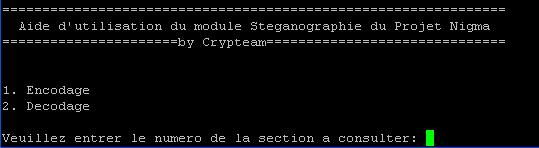
\includegraphics[scale=0.75]{aide1.JPG}
\end{center}

\begin{center}	
  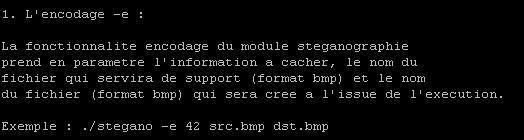
\includegraphics[scale=0.75]{aide3.JPG}
  \textit{\\En entrant le numéro de la section à consulter comme il est demandé, Serge pourra consulter l'aide sur l'encodage}
\end{center}

\begin{center}	
  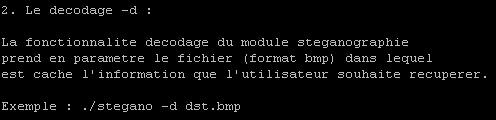
\includegraphics[scale=0.75]{aide2.JPG}
  \textit{\\Et pour Jeanne il y'a l'aide sur le décodage}
\end{center}

L'aide utilisateur va donc décrire les deux utilisations du programme : encodage et décodage, en indiquant les paramètres de chacune et en mettant à disposition un exemple d'utilisation.

Un peu de Code à présent !

La fonction de décodage est construite sur deux boucles : la première est chargée de sauter le header afin de traiter uniquement les pixels codés, la seconde a pour but de traiter chaque pixel de l'image jusqu'à ce qu'elle rencontre un pixel blanc.
Dans un premier temps la fonction principale du décodage fût la suivante :

\begin{small}
  \begin{verbatimtab}
    char *decode (char *name)
    {
      FILE *src;
      char *res;
      int go_print;
      int jump ;
      int bit_uncoded ;
      pixel bit_coded ;
      res = calloc(1,1);
      jump = 0;
      bit_coded.blue=0;
      bit_coded.green = 0;
      bit_coded.red = 0;
      src = fopen(name,"r");
      for(jump = 0;jump != 54;jump++)
      {
        bit_uncoded = getc(src);
      }
      while(bit_coded.blue == 255 && bit_coded.green == 255
            && bit_coded.red == 255)
      {
        bit_coded.blue = getc(src);
        bit_coded.green = getc(src);
        bit_coded.red = getc(src);
        res = strcat(res,pix_to_bit(bit_coded.blue));
        res = strcat(res,pix_to_bit(bit_coded.green));
        res = strcat(res,pix_to_bit(bit_coded.red));
      }
      fclose(src);
      return(res);
    }
  \end{verbatimtab}
\end{small}

Où pix\_to\_bit est la fonction qui transforme une valeur R, G ou B d'un pixel en un 0 ou un 1 comme expliqué précédemment :

\begin{small}
  \begin{verbatimtab}
    char *pix_to_bit (int val)
    {
      if(val % 2 == 0)
      {
        return("0");
      }
      else
      {
        return("1");
      }
    }
  \end{verbatimtab}
\end{small}

Mais nous avons rencontrés un problème à cause du cas d'arrêt :

\begin{small}
  \begin{verbatimtab}
    (bit_coded.blue == 255 && bit_coded.green == 255
     && bit_coded.red == 255)
  \end{verbatimtab}
\end{small}

En effet la boucle traitait le pixel blanc comme un pixel normal, la fonction renvoyait de manière systématique 111 à la fin de la chaîne de bits. Pour pallier à ce problème j'ai crée une variable entière go\_print que j'ai utilisé à la manière d'un booléen (les booléens nécessitant l'utilisation d'une bibliothèque spécifique en C) pour forcer le programme à ne pas traiter le dernier pixel. La nouvelle boucle est donc :

\begin{small}
  \begin{verbatimtab}
    int go_print;
    /* déclaration et initialisation de la nouvelle variable */
    go_print = 1;

    while(go_print)
    {
      bit_coded.blue = getc(src);
      bit_coded.green = getc(src);
      bit_coded.red = getc(src);
      if(bit_coded.blue == 255 && bit_coded.green == 255
         && bit_coded.red == 255)
      {
        go_print = 0;
      }
      else
      {
        res = strcat(res,pix_to_bit(bit_coded.blue));
        res = strcat(res,pix_to_bit(bit_coded.green));
        res = strcat(res,pix_to_bit(bit_coded.red));
      }
    }
    fclose(src);
    return(res);
    }
  \end{verbatimtab}
\end{small}

Finalement une fois le principe de notre module de stéganographie établit avec l'aide de Justin ainsi que l'encodage réalisé par ce même comparse, il n'a pas été très difficile de faire la fonction inverse (mis à part le problème mentionné ci-dessus). Le travail sur la stéganographie a surtout porté sur la mise en place du concept, sur le fonctionnement du format bitmap et sur le principe de la manipulation des pixels. Ainsi j'ai eu le temps d'aider mes deux collègues chargés de la cryptographie au niveau des maths fondamentales sur les tests de primalités et l'établissement des clés publiques et privées (algorithme d'Euler étendu).

\newpage

\section{Site Web}

Le site Web a été réalisé par Sébastien Gislais. Il a été codé en xHTML avec des CSS (feuilles de style) ainsi qu'en PHP. Notre site Web peut se mettre facilement à jour. Il est léger et possède une présentation très claire de notre projet. Il respecte bien entendu les normes et les recommandations du W3C pour une parfaite accessibilité.

\bigskip

Il est en ligne à cette adresse : \href{http://projetnigma.free.fr/}{http://projetnigma.free.fr/}

\bigskip

Nous avons une page de présentation de notre Team pour expliquer notre démarche et partager notre vécu à travers ce projet d'envergure. Dans le but de fournir une sorte de support aux visiteurs qui s'intéressent eux aussi à la cryptographie et à la stéganographie, nous avons mis en place une page de liens vers les sites indispensables que nous avons parcourus et appris par c\oe{}ur\dots{}

Les sources du projet sont disponibles et permettent d'autant plus de partager notre expérience avec le monde entier. Il est possible d'entrer en contact avec nous pour de plus amples informations ou conseils \emph{via} une messagerie électronique que nous laissons à disposition.

Le site Web est complet, continuera d'être mis à jour régulièrement et informera de l'avancée du projet durant l'année.

\newpage

\section{Conclusion}

Haut les c\oe{}urs ! Ce rapport de soutenance est bientôt achevé, nous voici arrivé à la conclusion ! Nous avons donc obtenu au cours de nos longues heures de travail assidues un programme tout à fait fonctionnel et prêt à l'utilisation, néanmoins il nous reste encore beaucoup à accomplir. En effet si le programme marche actuellement de façon tout à fait respectable, il reste de nombreuses améliorations à faire pour augmenter ses performances, sa fiabilité et son utilisation. Par exemple l'implémentation d'une interface graphique rendrait l'utilisation du Projet Nigma bien plus intuitive pour des utilisateurs lambda (comme Jeanne et Serge).

Pour ce qui est de la stéganographie, actuellement le programme prend en paramètre une chaîne de caractère pour la cacher au sein d'une image, c'est pratique pour faire passer des messages comme \og à quelle heure a lieu la soutenance ? \fg{} qui ne sont pas cryptés au préalable. Mais une fois le message crypté on obtient une suite de chiffres passablement indigeste qui est difficile à recopier c'est pourquoi à l'avenir le programme prendra en paramètre un fichier dans lequel est stocké le produit du cryptage. Ainsi l'utilisateur ne perdra pas la vue en essayant de recopier le message crypté sans faire de fautes (qui seraient fatal à la conservation du sens du message). Un des autres objectifs futurs de la section stéganographie est l'implémentation de nouvelles techniques de camouflage : à l'instant ou vous lisez ces lignes le programme de stéganographie utilise une unique technique qui consiste à cacher un caractère dans 3 pixels en faisant varier de 1 au maximum les champs de couleur RGB des pixels. Cette technique est très discrète puisque le changement est imperceptible à l'\oe{}il nu (mis à part peut-être pour Jim Ellison) mais elle est limitée au niveau de la capacité de stockage : un caractère étant codé sur 9 bits, on ne peut en cacher que 160\,000 (espaces compris) dans une image de format bitmap $800 \times 600$, à première vue cela semble énorme mais une fois un message crypté (en RSA par exemple) celui-ci voit son nombre de caractère augmenter de façon tout à fait impressionnante. Le but est donc de trouver d'autres techniques possédant un bon ratio discrétion/capacité afin de proposer à l'utilisateur une gamme de méthodes qui conviendront à différents usages (une personne voulant juste cacher une phrase n'utilisera pas la même technique de stéganographie que la personne voulant faire circuler un roman de manière illicite).

\bigskip

Du coté de la cryptographie, il nous reste pas mal de choses à faire. Nous avons prévu de faire du cryptage DES pour la deuxième soutenance. Le DES, contrairement au RSA, est un cryptage symétrique. Il n'y a donc qu'une seule clé permettant de chiffrer et de déchiffrer un document. Il possède un grand avantage par rapport au RSA : il est mille fois plus rapide ! Par contre le problème avec le DES c'est qu'il faut pouvoir envoyer cette clé au destinataire afin qu'il puisse chiffrer ses documents. Ce qui pose un problème : comment transmettre cette clé sans qu'il y ait de risque qu'elle soit récupérée par une personne mal intentionnée ? Ainsi, une des solutions envisageables est de chiffrer tout simplement cette clé avec par exemple\ldots{} le RSA ! C'est exactement comme cela que fonctionne les systèmes d'identification, les envois de code de carte de crédit, etc. Nous n'avons donc plus de problème au niveau de l'échange des clefs. Nous pourrons donc chiffrer notre document puis le cacher dans une image à l'aide de notre partie stéganographie ! Ainsi le message sera introuvable !

\newpage

\section{Annexe}

\begin{landscape}
  \subsection {Screenshot Cryptographie}
  \begin{center}
    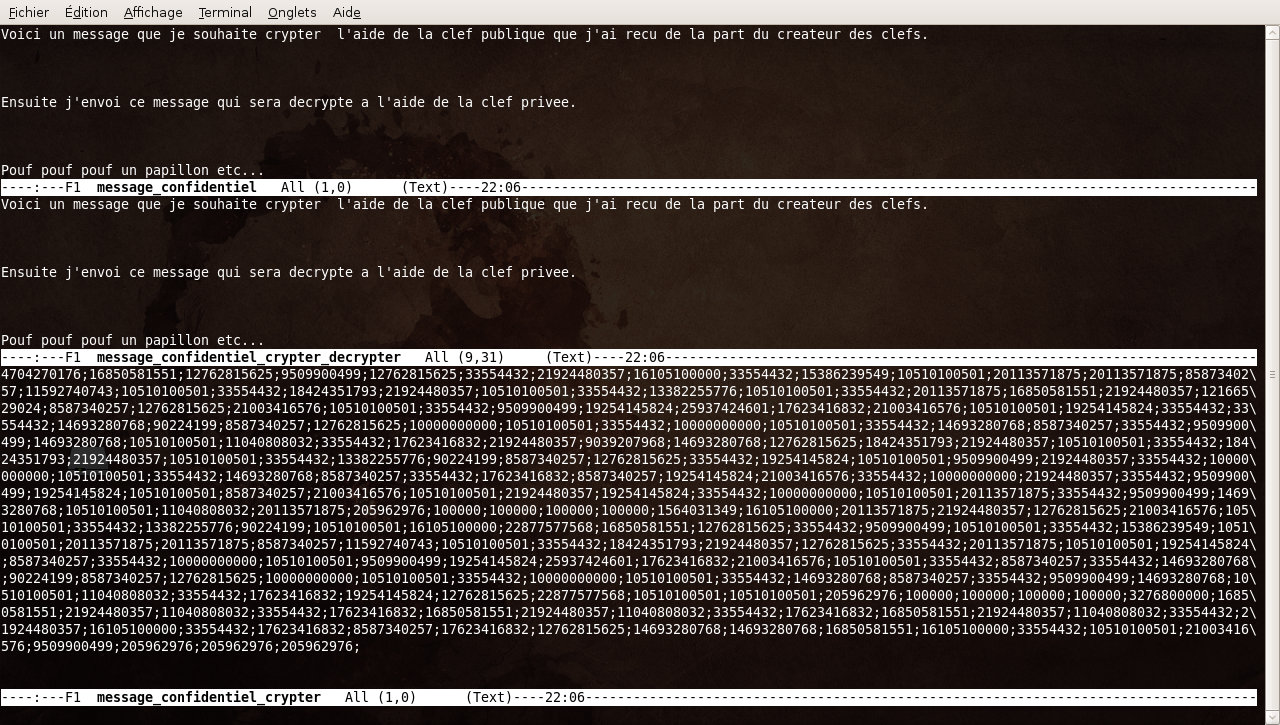
\includegraphics[scale=0.42]{cryptage.jpg}\\
    \textit{En haut le texte à chiffrer}\\
    \textit{Au milieu le texte chiffré puis déchiffré}\\
    \textit{En bas le texte chiffré}\\
  \end{center}
\end{landscape}

\newpage

\end{document}
